% !TeX root = thesis.tex

\chapter{Methodology} \label{chap:methodology}

This chapter describes the methodological approach adopted in this dissertation. It begins by describing 
the dataset used throughout this work and the exploratory data analysis conducted to characterize its 
main properties and challenges. It then details the data preprocessing pipeline applied prior to model 
development, including data cleaning, normalization, and sequence construction, followed by the specific 
formulation adopted for the AD, FD, and PdM tasks. The 
chapter subsequently describes the traditional ML baselines, single-task DL 
models, and multi-task DL architectures developed in this dissertation, together with the 
evaluation metrics used to compare them. 

\section{Dataset Description} \label{sec:dataset}

This section describes the dataset used throughout this dissertation. It first details how the data was 
acquired and the main limitations associated with its collection, and then presents the process variables 
included in the dataset together with their physical location within the plant and the vacuum pump.

\subsection{Data Acquisition} \label{sec:data_acquisition}

The dataset used in this dissertation was provided by Sysadvance and consists of real operational data 
collected from a VPSA biomethane upgrading plant located in Lithuania. Although the plant's sensors 
acquire measurements at a native sampling rate of 1 second, the dataset provided for this work was 
extracted from Sysadvance's database at 1-minute intervals, rather than at the sensors' native 
resolution. The dataset spans a period of approximately one month, from 11 March to 10 April, contains 
40{,}773 observations and was supplied in Microsoft Excel (\texttt{.xlsx}) format.

The company only started monitoring this specific vacuum pump partway through the data collection period. 
Consequently, the process variables associated with the general plant operation (FT-201, FT-801, FT-901, 
PT-901, PT-902, and Mode) are available from the beginning of the collection period, whereas the 
pump-specific variables (PT-903, TT-901 to TT-904, VSD-901\_CORRENT, VSD-901\_POWER, VSD-901\_RPM, 
VSD-901\_SPEED, and LS-901) only contain valid readings from a later point onward. This is addressed 
during the the data cleaning step.

According to Sysadvance, no vacuum pump fault occurrences have been recorded across any of their 
monitored plants to date. Consequently, the dataset used in this dissertation corresponds exclusively 
to normal operating conditions, and fault scenarios relevant to this work were synthetically injected by 
manipulating the collected variables, following the common failure modes identified in the 
manufacturer's troubleshooting guide.

No records of maintenance interventions performed during plant stoppages were available for this dataset, 
making it impossible to determine whether specific actions, such as filter replacement, were carried out 
during any given downtime period, which would in turn affect the physical condition of the equipment 
being measured. For the purposes of this dissertation, it is assumed that the inlet, exhaust, and oil 
filters were replaced jointly with the lubricating oil, in accordance with the manufacturer's recommended 
maintenance schedule and that the equipment therefore operated under 
nominal physical conditions throughout the collection period.

The plant's SCADA system collects several dozen process variables in total. However, only the subset 
presented in Table~\ref{tab:dataset_variables} was made available for this dissertation, selected by 
Sysadvance as the variables most directly relevant to the vacuum pump's condition monitoring.

\begin{table}[htbp]
\centering
\caption{Process variables included in the original dataset.}
\label{tab:dataset_variables}

\begin{tabular}{lll}
\hline
\textbf{Tag} & \textbf{Description} & \textbf{Unit} \\
\hline
FT-201           & Biogas inlet flow                     & Nm$^3$/h \\
FT-801           & Biomethane outlet flow                & Nm$^3$/h \\
FT-901           & Exhaust gas flow                       & Nm$^3$/h \\
Mode             & Run mode                               & integer \\
PT-901           & Gas line inlet vacuum pressure         & bar \\
PT-902           & Gas line outlet vacuum pressure        & bar \\
PT-903           & Vacuum pressure in oil separator       & bar \\
TT-901           & Oil separator gas temperature          & $^\circ$C \\
TT-902           & Discharge 1 temperature                & $^\circ$C \\
TT-903           & Discharge 2 temperature                & $^\circ$C \\
TT-904           & Oil temperature                        & $^\circ$C \\
VSD-901\_CORRENT & Vacuum pump current                    & A \\
VSD-901\_POWER   & Vacuum pump power                      & W \\
VSD-901\_RPM     & Vacuum pump rotation                   & RPM \\
VSD-901\_SPEED   & Vacuum pump speed                      & \% \\
LS-901           & Oil level sensor                       & true/false \\
\hline
\end{tabular}
\end{table}

\subsection{Process Variables} \label{sec:process_variables}

Figure~\ref{fig:plant pid} presents a simplified process flow diagram identifying the position of the 
process variables located outside the vacuum pump. The biogas inlet flow (FT-201) is measured upstream 
of the adsorption beds, while the biomethane outlet flow (FT-801) is measured downstream. 
The vacuum line inlet pressure (PT-901) is measured immediately before the vacuum pump, and the 
vacuum line outlet pressure (PT-902) and exhaust gas flow (FT-901) are measured immediately after it. The 
diagram also identifies the recovered gas stream, corresponding to the small fraction of methane 
desorbed during the initial seconds of the vacuum stage, which is redirected back to the biogas inlet 
rather than discharged as exhaust, as previously described.

\begin{figure}[htbp]
    \centering
    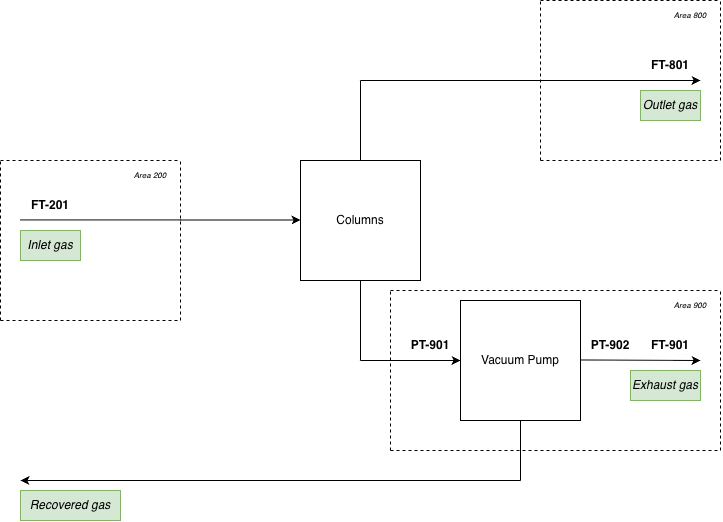
\includegraphics[width=0.85\textwidth]{imgs/plant pid.png}
    \caption{Simplified process flow diagram identifying the position of the monitored process variables.}
    \label{fig:plant pid}
\end{figure}

The remaining process variables are associated with the internal operation of the vacuum pump itself, 
namely the oil separator pressure and gas temperature (PT-903 and TT-901), the discharge temperatures 
(TT-902 and TT-903), the oil temperature (TT-904), the oil level sensor (LS-901), and the electrical and 
mechanical variables of the pump motor (VSD-901\_CORRENT, VSD-901\_POWER, VSD-901\_RPM, and VSD-901\_SPEED). 
The physical location of these internal components was already presented in 
Section~\ref{sec:components} and illustrated in Figures~\ref{fig:vacuumoperation} and~\ref{fig:vacuumpump}.

Unlike the remaining continuous process variables, \texttt{Mode} is a 
categorical variable describing the operating state of the system rather than a continuously measured 
physical quantity. Among its possible values, only modes 8 and 9 correspond to the plant's production 
state. The remaining values, whose exact meaning was not disclosed by Sysadvance, correspond to 
non productive states and are therefore not relevant to this dissertation.

\section{Exploratory Data Analysis} \label{sec:eda}

This section characterizes the behaviour of the variables prior to any filtering or 
preprocessing, in order to identify patterns and challenges relevant to subsequent modelling decisions. 
Time series plots and distribution histograms for all remaining continuous process variables not shown 
in this section are provided in Appendix~\ref{ap1:eda_plots} for completeness.

This late start to the pump monitoring, affects 
1{,}598 of the 40{,}773 total observations, all of them at the very beginning of the collection period. 
The analysis in this section is therefore based on the remaining observations, from the point onward 
where all sensors report valid readings.

The continuous process variables were characterized over the entire collection period, as summarized in 
Table~\ref{tab:eda_summary}. The vacuum line pressures (PT-901, PT-902) show negative values, which makes 
sense given that the pump operates below atmospheric pressure during the vacuum stage of the VPSA cycle. 
The pump's electrical and mechanical variables drop to zero only outside the plant's production modes, 
which lines up with the pump simply being off rather than any faulty readings.

VSD-901\_RPM and VSD-901\_SPEED also stand out for having a very tight IQR, since the pump barely 
deviates from its setpoint once running. Because of this, even small, harmless fluctuations get flagged 
as outliers under the IQR rule, which explains why these two variables show the highest outlier 
percentages in the table despite not reflecting any real fault.

The negative minimum values seen for FT-201 and FT-801 don't make physical sense for a flow measurement 
and are treated accordingly during the data cleaning stage.

\begin{table}[htbp]
\centering
\caption{Descriptive statistics and IQR-based outlier proportions for the continuous process variables 
(full dataset, all operating modes).}
\label{tab:eda_summary}
\scriptsize
\begin{tabular}{lrrrrrrrr}
\hline
\textbf{Tag} & \textbf{Mean} & \textbf{Std} & \textbf{Min} & \textbf{Q1} & \textbf{Median} & \textbf{Q3} & \textbf{Max} & \textbf{Outliers (\%)} \\
\hline
PT-901           & -0.681  & 0.249  & -1.025  & -0.833  & -0.721  & -0.552  & 0.088    & 3.69  \\
PT-902           & 0.014   & 0.012  & -0.014  & 0.006   & 0.011   & 0.020   & 0.051    & 3.38  \\
PT-903           & 0.066   & 0.265  & -2.896  & 0.050   & 0.081   & 0.126   & 0.259    & 1.34  \\
TT-901           & 67.06   & 5.05   & 18.39   & 64.71   & 67.49   & 69.95   & 77.08    & 1.48  \\
TT-902           & 68.25   & 4.96   & 19.12   & 65.95   & 68.63   & 71.09   & 78.11    & 1.42  \\
TT-903           & 77.24   & 5.23   & 21.42   & 74.63   & 77.70   & 80.18   & 88.40    & 1.40  \\
TT-904           & 77.01   & 5.49   & 18.36   & 74.57   & 77.47   & 79.94   & 87.92    & 1.59  \\
FT-201           & 621.79  & 160.07 & -15.06  & 597.09  & 652.13  & 718.82  & 826.26   & 9.96  \\
FT-801           & 308.18  & 87.33  & -800.00 & 303.59  & 328.64  & 352.56  & 760.18   & 7.89  \\
FT-901           & 307.04  & 235.33 & 2.25    & 159.29  & 266.70  & 434.98  & 929.00   & 3.58  \\
VSD-901\_CORRENT & 43.03   & 10.15  & 0.00    & 42.93   & 47.13   & 49.71   & 53.70    & 18.28 \\
VSD-901\_POWER   & 24.33   & 9.09   & 0.00    & 25.48   & 28.51   & 30.20   & 33.05    & 21.13 \\
VSD-901\_RPM     & 1069.36 & 281.26 & 0.00    & 1198.83 & 1199.71 & 1200.51 & 1211.72  & 22.42 \\
VSD-901\_SPEED   & 89.12   & 23.43  & 0.00    & 99.97   & 100.00  & 100.01  & 100.79   & 24.84 \\
\hline
\end{tabular}
\end{table}

Beyond these summary numbers, the data also shows a clear cyclic pattern tied to the VPSA process. A few 
hours of PT-901 data, shown in the top panel of Figure~\ref{fig:eda_pt901_cycle}, make the switching 
between the four adsorption columns clearly visible: the vacuum 
pressure measured at the gas line inlet rises and falls repeatedly rather than settling at a single value. 
The distributions in the bottom panels show a similar pattern for PT-901 and PT-902, both located along 
the gas line, while PT-903, measured inside the oil separator, shows a narrower, more concentrated 
distribution.

\begin{figure}[htbp]
    \centering
    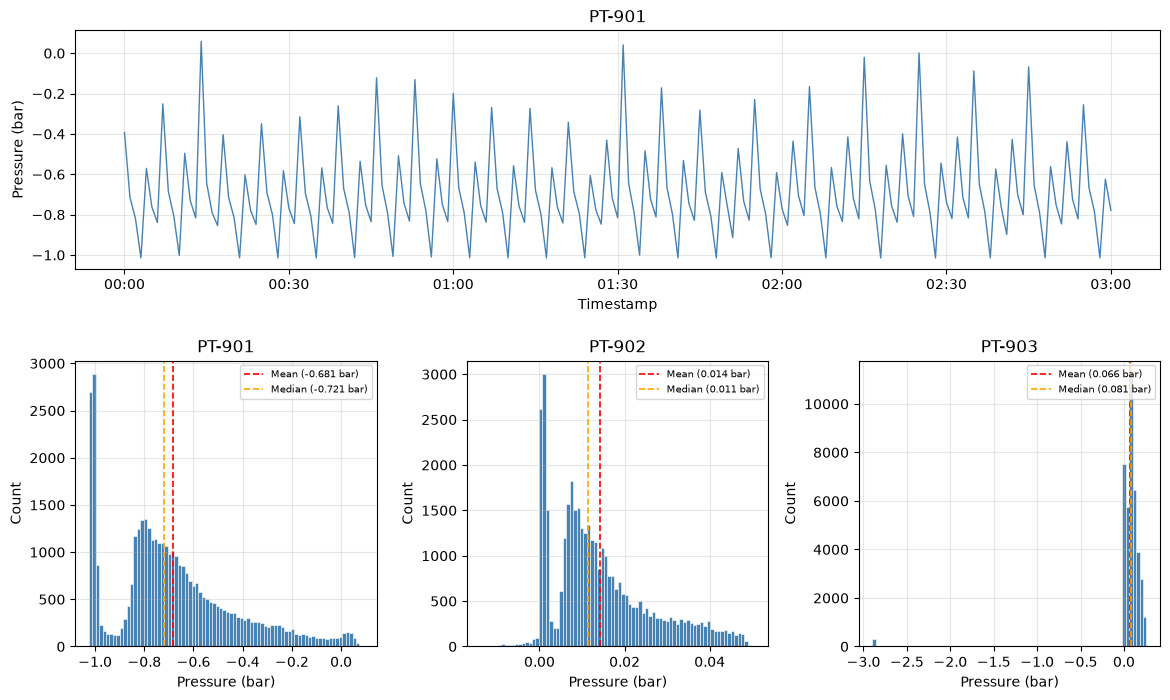
\includegraphics[width=0.95\textwidth]{imgs/eda_pt901_cycle_and_distributions.png}
    \caption{Top: excerpt of PT-901 showing the repeating pattern associated with the VPSA cycle. Bottom: 
    distributions of the three vacuum pressure sensors (PT-901, PT-902, PT-903).}
    \label{fig:eda_pt901_cycle}
\end{figure}

A small, isolated cluster of 294 consecutive observations near $-2.9$~bar is also visible for PT-903. 
Further inspection revealed that this cluster corresponds to a single continuous episode, spanning 
approximately five hours (04:11 to 09:09 on 7 April), during which the sensor reading remained frozen at 
exactly the same value ($-2.896296$~bar), as shown in Figure~\ref{fig:eda_pt903_frozen}. Although the 
vacuum pump's power draw was initially low for part of this episode, it recovered to typical operating 
levels around 8:00, while PT-903 remained frozen at the same constant value until 09:09. Since a genuine 
pressure reading would be expected to vary once the pump resumed normal operation, this behaviour is 
attributed to a sensor or data acquisition fault rather than to the pump simply being idle.

\begin{figure}[htbp]
    \centering
    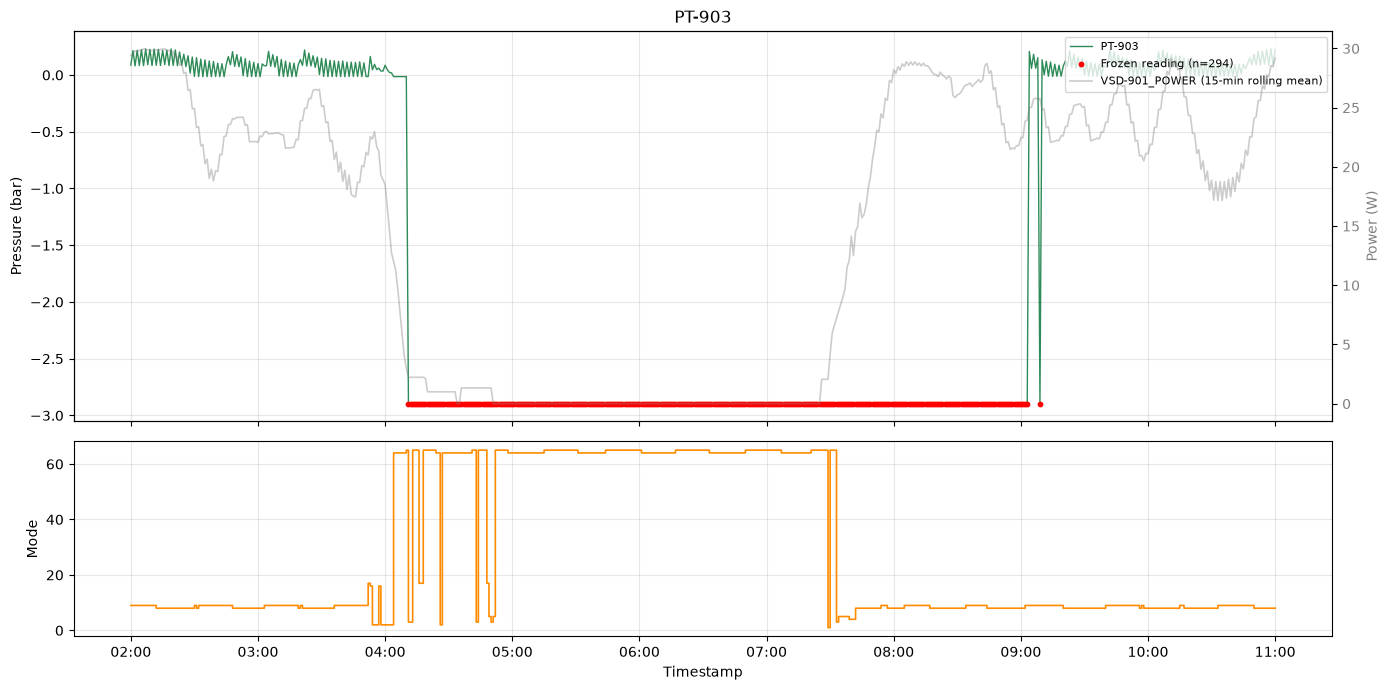
\includegraphics[width=0.95\textwidth]{imgs/eda_pt903_frozen.png}
    \caption{Top: PT-903 around the frozen sensor episode on 7 April, with the affected observations 
    highlighted and the vacuum pump power (15-minute rolling mean) overlaid on a secondary axis. Bottom: 
    the plant's operating mode over the same period.}
    \label{fig:eda_pt903_frozen}
\end{figure}

A closer look at FT-801 also revealed 27 observations reading exactly $-800.000000$, each occurring in 
isolation at a different point in time rather than as part of a single, sustained episode. Given its 
constant, round number and its physical implausibility, this reading is treated as invalid during data 
cleaning, regardless of its underlying cause.

Beyond these value issues, the timestamps themselves are not perfectly continuous either. An 
analysis of the timestamp continuity revealed 77 gaps larger than 1 minute across the entire collection 
period, together accounting for 1 day, 16 hours, and 3 minutes of missing time, roughly 5.6\% of the 
total collection period. Table~\ref{tab:eda_gaps} breaks these gaps down by duration. The majority are 
brief: 33 gaps last between 1 and 5 minutes and 37 last between 5 and 30 minutes, most likely 
corresponding to short communication interruptions with the database rather than actual plant stoppages. 
Only 7 gaps exceed 30 minutes, ranging from 48 minutes to over 10 hours, making these the ones most 
likely to reflect genuine plant stoppages.

\begin{table}[htbp]
\centering
\caption{Distribution of timestamp gaps larger than 1 minute across the collection period.}
\label{tab:eda_gaps}
\begin{tabular}{lr}
\hline
\textbf{Gap duration} & \textbf{Count} \\
\hline
1--5 min    & 33 \\
5--30 min   & 37 \\
30 min--2 h & 3  \\
2--12 h     & 4  \\
$>$12 h     & 0  \\
\hline
\textbf{Total} & \textbf{77} \\
\hline
\end{tabular}
\end{table}

These 7 largest gaps, together with the plant's production operating mode (Mode 8 or 9), are highlighted 
in Figure~\ref{fig:eda_gaps_overview} against the vacuum pump current over the full collection period.

\begin{figure}[htbp]
    \centering
    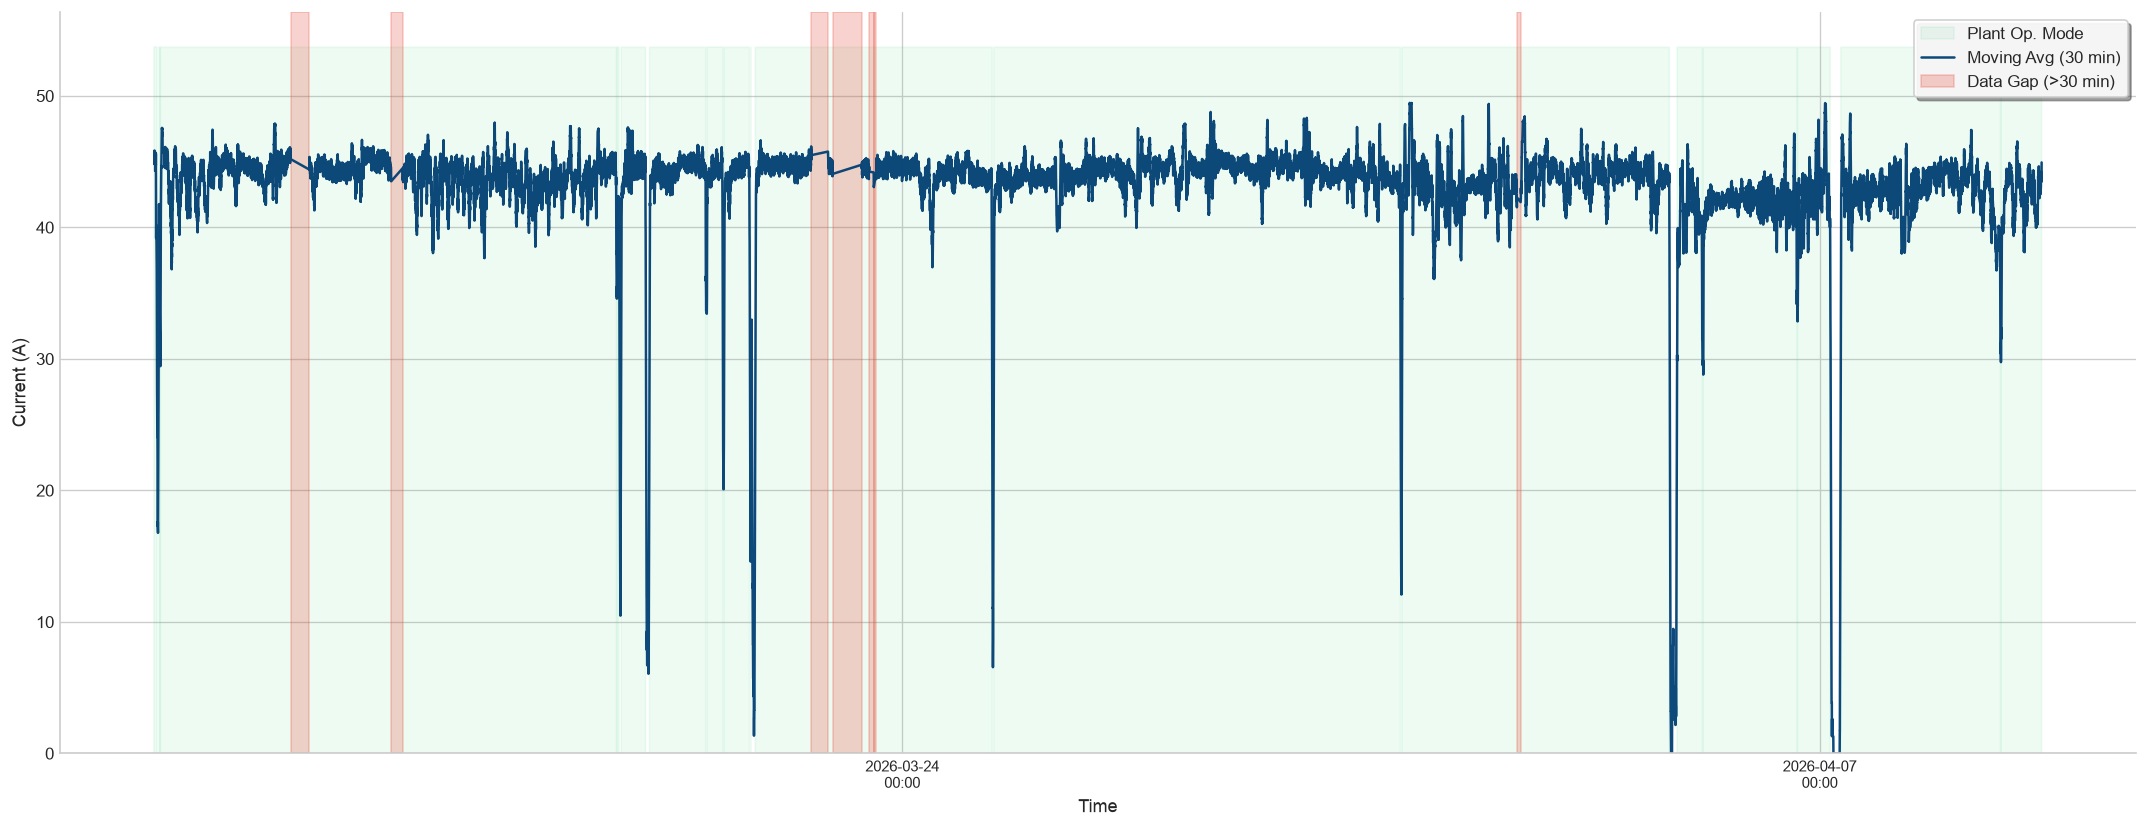
\includegraphics[width=0.95\textwidth]{imgs/eda_gaps_overview.png}
    \caption{30-minute moving average of the vacuum pump current (VSD-901\_CORRENT) across the full 
    collection period, with the 7 largest data gaps (red) and the plant's production operating mode 
    (green) highlighted.}
    \label{fig:eda_gaps_overview}
\end{figure}

Finally, the relationships between variables were also examined, restricting the analysis to the plant's 
production modes. As expected from the physical relationship between the pump motor's 
electrical and mechanical behaviour, the current, power, rotational speed, and percentage speed variables 
(VSD-901\_CORRENT, VSD-901\_POWER, VSD-901\_RPM, VSD-901\_SPEED) show strong positive correlation with 
one another, as seen in Figure~\ref{fig:eda_correlation}. Similarly, the discharge and oil temperatures 
(TT-901, TT-902, TT-903, TT-904) show a strong positive relationship, reflecting shared thermal dynamics within 
the pump.

\begin{figure}[htbp]
    \centering
    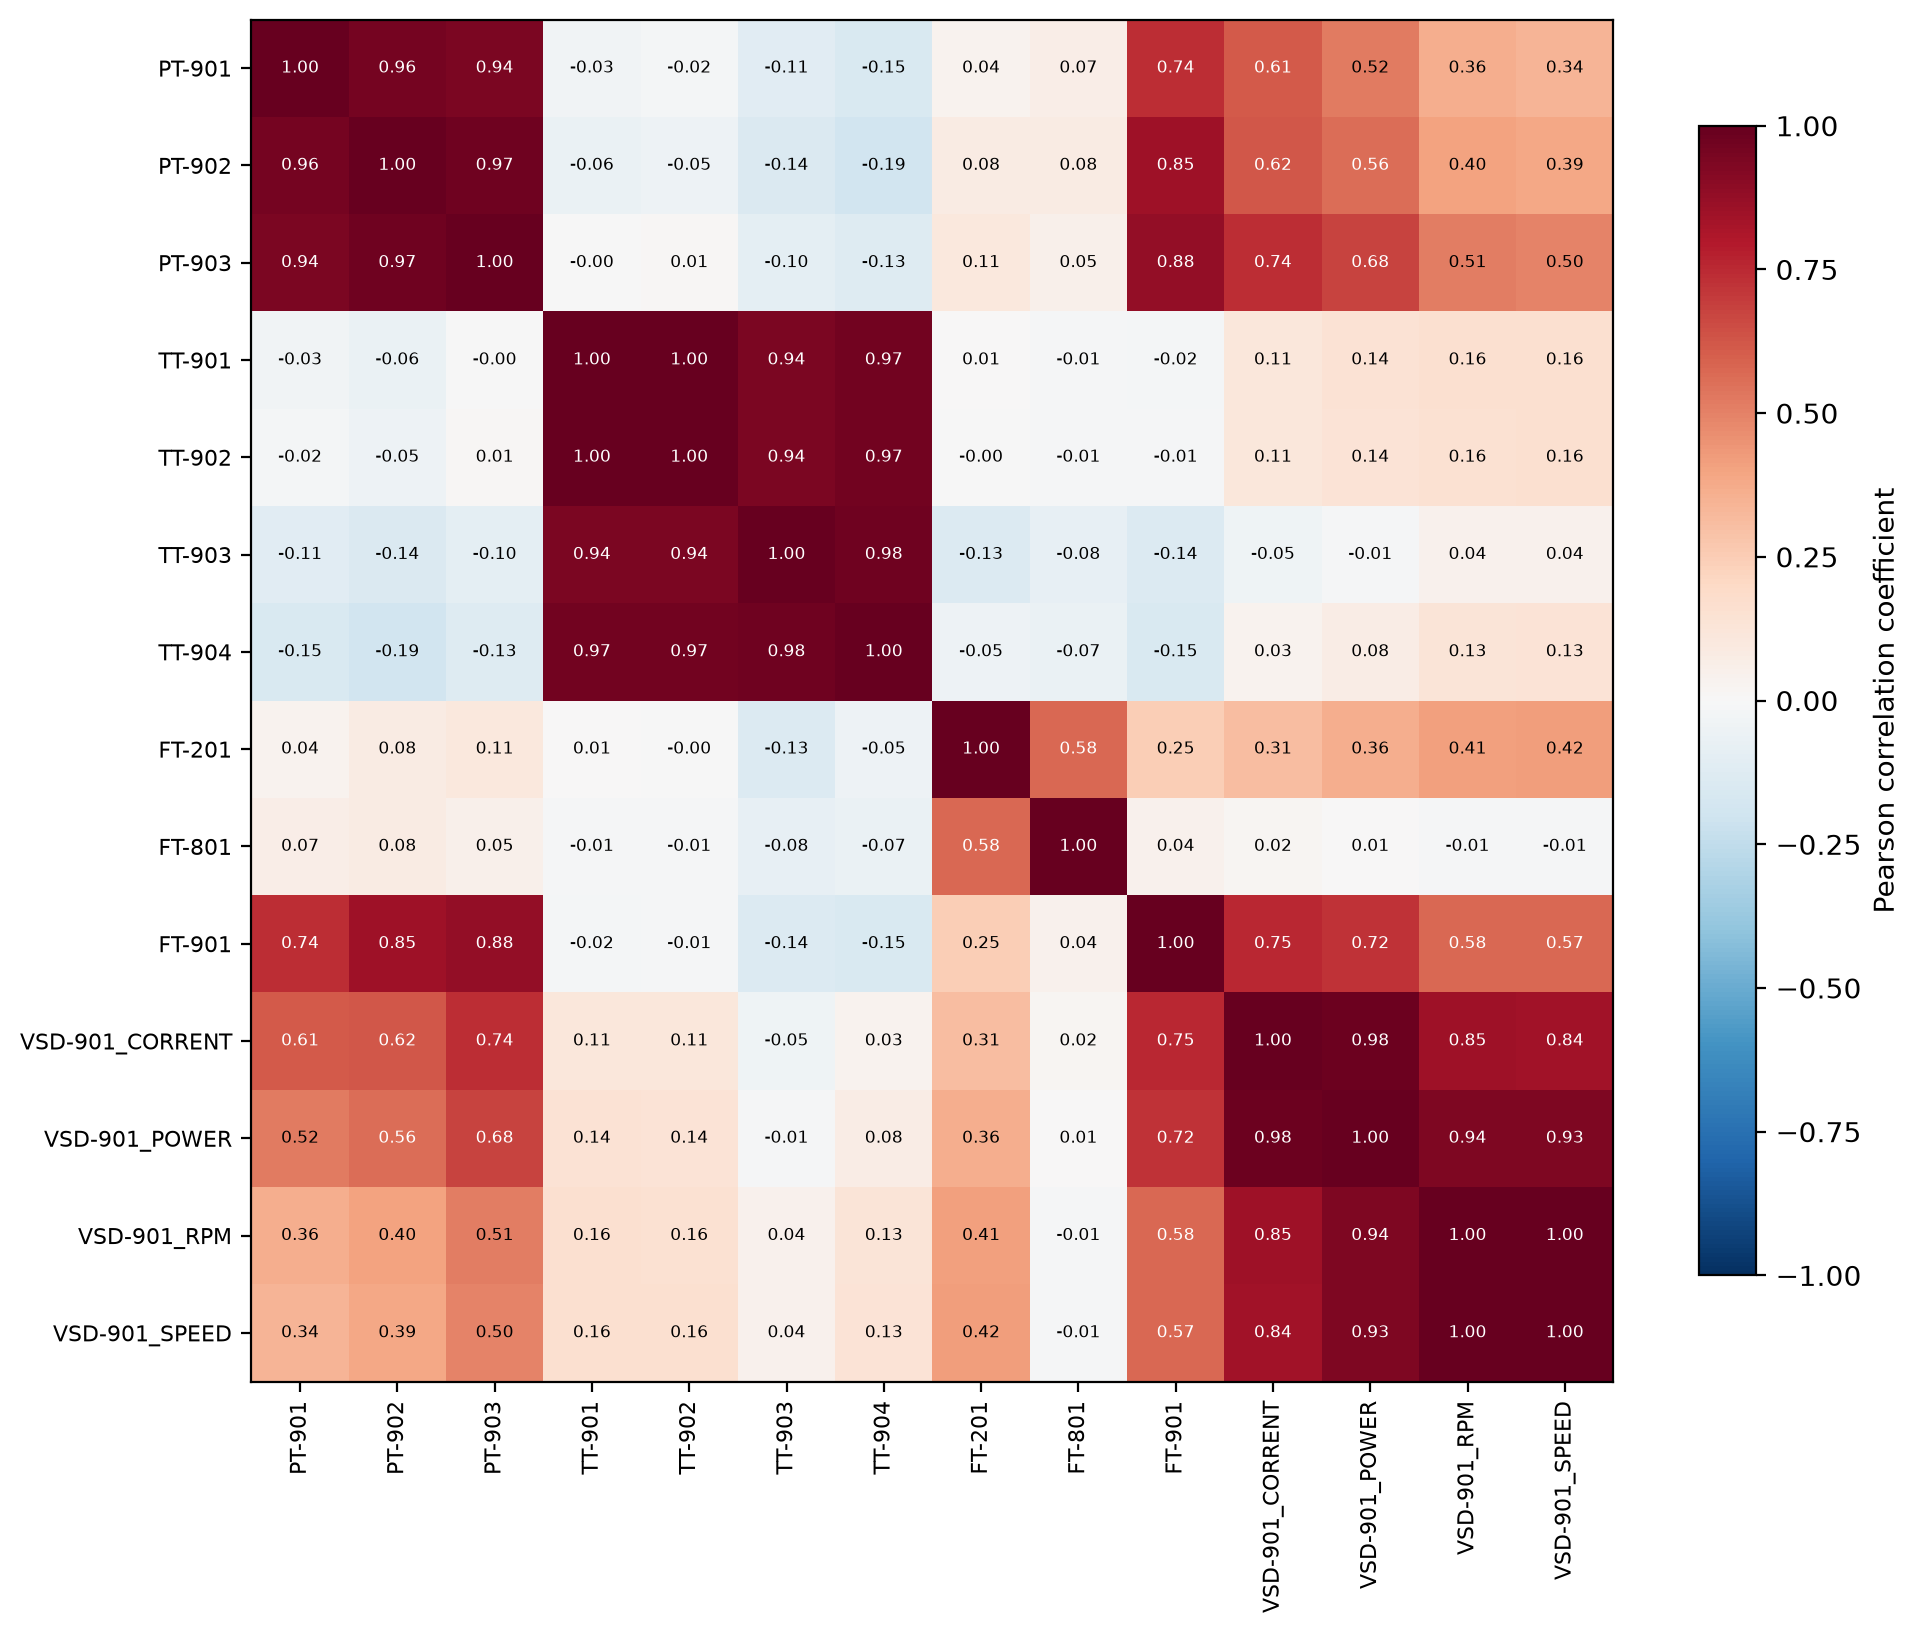
\includegraphics[width=0.85\textwidth]{imgs/eda_correlation_matrix.png}
    \caption{Correlation matrix of the continuous process variables, restricted to production modes 
    (Mode 8 and 9).}
    \label{fig:eda_correlation}
\end{figure}

\section{Data Cleaning} \label{sec:cleaning}

The raw dataset, comprising 40{,}773 observations, was processed through a sequence of cleaning steps 
prior to feature engineering and model development.

First, the leading observations preceding the point at which all sensors had begun reporting valid 
readings were removed, reducing the dataset from 40{,}773 to 39{,}175 observations. Second, the 27 
isolated FT-801 readings of exactly $-800.000000$ previously identified were invalidated. 
Since each of these occurs in isolation, at a single minute rather than as part of a sustained episode, 
they were not removed as separate rows but instead left to be filled in through the same linear 
interpolation step applied to short timestamp gaps within each session, described later in this section.

In contrast, the frozen PT-903 sensor episode was deliberately 
retained rather than removed or corrected. Since this episode reflects a known instrumentation fault 
rather than a genuine change in the pump's condition, it provides a useful reference case for evaluating 
whether the anomaly detection models developed in this dissertation can be misled 
into raising a false positive. To support this later use, a binary flag column 
(\texttt{pt903\_frozen\_flag}) was added to the dataset, marking every observation belonging to this 
episode.

The dataset was then filtered to retain only observations corresponding to the plant's production modes. 
Prior to this filtering, the oil level sensor (LS-901) contained some missing values and was forward and backward filled 
across the entire dataset, since the lubricating oil level does not change simply because the sensor 
failed to report a reading.

The gaps identified in Section~\ref{sec:eda} differ substantially in likely cause and duration, ranging 
from brief communication interruptions of a few minutes to stoppages of several hours. While it is 
reasonable to assume that the plant's behaviour changes little across a short gap, making linear 
interpolation a safe approximation, the same cannot be assumed across gaps of several hours. During such 
an interval, the pump may have been shut down, restarted, or brought through an atypical start-up 
sequence, none of which can be reliably inferred from the surrounding data. Interpolating across such 
gaps would therefore risk fabricating a smooth, continuous transition that never actually occurred, which 
can be problematic for the models developed in this dissertation, since their 
core assumption is that consecutive time steps reflect a genuine, continuous evolution of the process. 
To avoid this, the data was split into independent sessions, with a new session 
boundary defined whenever a gap larger than 30 minutes was observed. This threshold separates the brief, 
interpolation safe interruptions from the longer gaps most likely to correspond to genuine plant 
stoppages. A session identifier column (\texttt{bucket\_id}) was added to the dataset to record this 
partitioning.

Within each resulting session, the data was resampled to a strict 1-minute frequency and linear 
interpolation was applied to fill in any remaining small gaps, including the invalidated FT-801 readings 
described above. 
Sessions containing fewer than 1{,}000 observations were discarded, as they were considered too short to 
be useful for the models developed, a decision revisited in Section~\ref{sec:windowing}.

This process yielded 18 candidate sessions, of which 11 met the minimum length requirement and were 
retained for subsequent analysis, totalling 37{,}376 observations. Table~\ref{tab:cleaning_sessions} 
summarizes the resulting sessions.

\begin{table}[htbp]
\centering
\caption{Production sessions retained after data cleaning.}
\label{tab:cleaning_sessions}
\small
\begin{tabular}{clrr}
\hline
\textbf{Session} & \textbf{Period} & \textbf{Observations} \\
\hline
1  & 03-12 15:38 to 03-14 15:57 & 2{,}900 \\
2  & 03-14 22:50 to 03-16 04:48 & 1{,}799 \\
3  & 03-16 09:02 to 03-19 16:24 & 4{,}763 \\
5  & 03-20 03:25 to 03-21 06:10 & 1{,}606 \\
8  & 03-21 18:10 to 03-22 14:44 & 1{,}235 \\
12 & 03-23 14:22 to 03-25 08:57 & 2{,}556 \\
13 & 03-25 09:31 to 03-31 14:28 & 8{,}938 \\
14 & 03-31 15:00 to 04-02 09:06 & 2{,}527 \\
15 & 04-02 10:28 to 04-04 16:57 & 3{,}270 \\
16 & 04-04 19:45 to 04-07 03:51 & 3{,}367 \\
17 & 04-07 07:42 to 04-10 09:16 & 4{,}415 \\
\hline
\textbf{Total} & & \textbf{37{,}376} \\
\hline
\end{tabular}
\end{table}

\section{Fault Injection} \label{sec:fault_scenarios}

As previously established, no vacuum pump fault occurrences have been recorded 
by Sysadvance across any of their monitored plants. Consequently, fault scenarios relevant to the AD, FD, 
and PdM tasks addressed in this dissertation were synthetically injected into two of the eleven 
sessions retained after data cleaning: Session 16 and Session 17.

These two sessions were selected primarily because using more than one session, rather than concentrating 
all fault injection in a single one, exposes the models to two distinct underlying data 
distributions rather than just one, even if the difference between them is modest. This is intended to 
support better generalization when evaluating model performance, avoiding a scenario in which all fault 
examples are drawn from a single continuous stretch of plant behaviour. Sessions 16 and 17 were judged to 
have an acceptable length and observation count for this purpose.

All fault scenarios follow a common approach: rather than injecting a fixed, absolute signal deviation, 
each injected fault is calibrated against the behaviour the affected sensor exhibits in that same session. 
The target value the sensor is driven towards is defined by the manufacturer's warning and trip 
thresholds, as described in Section~\ref{sec:fault_severity}, and is therefore the same across sessions. 
What varies between sessions is the deviation required to reach it: this is obtained from the difference 
between that target and the sensor's mean value over the portion of the session preceding the fault 
window, excluding any observations belonging to the frozen PT-903 episode, whose constant reading would 
otherwise bias the estimate. The standard deviation over the same observations sets the amplitude of the 
stochastic noise superimposed on the injected signal, so that the noise remains proportionate to the 
sensor's own natural variability rather than being fixed at an arbitrary level. A fault injected into a 
session where the sensor was already running slightly high therefore requires a correspondingly smaller 
deviation than the same fault injected into a session where it was running low, while both end up 
reaching the same target.

\subsection{Severity Levels} \label{sec:fault_severity}

Three severity levels, small, medium, and severe, were defined for each fault scenario, based on the
warning and trip thresholds specified in the manufacturer's manual. Rather than being defined relative to
each sensor's own baseline, all three levels are anchored to the same reference interval, the distance
between the warning and trip thresholds of the affected sensor, as summarized in
Table~\ref{tab:fault_severity}. This makes a given severity level directly comparable across the four
fault scenarios, even though they act on sensors measuring different physical quantities over very
different numerical ranges: a medium fault always represents the same relative position within the
sensor's own alarm band, whether that band spans $0.1$~bar or $20\,^\circ$C.

\begin{table}[htbp]
\centering
\caption{Definition of fault severity levels relative to the manufacturer's warning and trip thresholds.
$\Delta$ denotes the distance between the two thresholds.}
\label{tab:fault_severity}
\begin{tabular}{lll}
\hline
\textbf{Severity} & \textbf{Target value} & \textbf{Position} \\
\hline
Small  & Warning threshold $+$ 25\% of $\Delta$ & Just past the warning threshold \\
Medium & Warning threshold $+$ 75\% of $\Delta$ & Approaching the trip threshold \\
Severe & Trip threshold $+$ 10\% of $\Delta$    & Beyond the trip threshold \\
\hline
\end{tabular}
\end{table}

The target value defines the peak of the injected deviation: the injected signal is scaled so that the
affected sensor reaches this value at the point where the deviation is largest, and stays below it
elsewhere within the fault window. A small fault therefore crosses the warning threshold but never
reaches the trip threshold, a medium fault approaches the trip threshold without crossing it, and a
severe fault crosses it.

Because the three levels differ only in where they land within a narrow alarm band, the smaller
severities remain harder to distinguish from normal operating variation than the severe ones,
particularly for sensors whose natural fluctuation is comparable to the width of the band itself. This is
an intentional part of the design: as previously discussed, the anomaly detection task considered in this
dissertation is not only about recognizing clearly abnormal behaviour, but also about assessing how
early a developing fault can be reliably identified.

\subsection{Fault Scenarios} \label{sec:fault_single}

Four fault scenarios were defined, each corresponding to a distinct failure mode identified in the 
manufacturer's troubleshooting guide. Table~\ref{tab:fault_types} summarizes the four fault types, their 
main sensor, and the shape of the signal deviation used to represent each one.

\begin{table}[htbp]
\centering
\caption{Fault scenarios and their main sensor and injected signal shape.}
\label{tab:fault_types}
\small
\begin{tabular}{p{1cm}p{3.3cm}p{2cm}p{6cm}}
\hline
\textbf{ID} & \textbf{Fault} & \textbf{Main sensor} & \textbf{Injected signal shape} \\
\hline
F1 & Clogged exhaust filters & PT-903 & Stochastic ramp with increasing 
noise, reflecting a gradual pressure build-up \\
F2 & Insufficient cooling & TT-901 & Stochastic ramp, analogous to F1, reflecting a gradual 
temperature increase \\
F3 & Float valve fault & PT-903 & Growing sinusoidal oscillation, reflecting the intermittent, 
chattering behaviour expected from a malfunctioning float valve rather than a monotonic drift \\
F4 & Defective bearing & TT-904 & Localized Gaussian temperature spike of short duration, reflecting a 
brief, sharp thermal event rather than a sustained drift \\
\hline
\end{tabular}
\end{table}

F1 and F2 are modelled as gradually developing faults, consistent with the progressive nature of filter 
clogging and cooling degradation: the ramp is combined with 
increasing stochastic noise, so that the signal becomes progressively less stable as the fault develops. 
In contrast, F3 is modelled as an oscillation between the baseline and the severity target rather than a 
monotonic ramp, since a malfunctioning float valve is expected to produce intermittent, chattering 
pressure fluctuations rather than a steady drift. F4 differs from the other three in both shape and duration: rather than 
developing gradually over several hours, it is modelled as a short, localized temperature spike, 
consistent with the more abrupt thermal signature expected from a defective bearing.

For each fault, the injected deviation is applied to the main sensor and also propagated to the process
variables correlated with it, so that the fault does not appear as an implausible event affecting a single
measurement. A variable counts as correlated when its absolute Pearson correlation with the main sensor
reaches 0.70 for the pressure related faults, or 0.60 and 0.65 for the temperature related faults,
computed on that session's own data before injection and excluding the frozen PT-903 episode. The main
sensor receives the full deviation, while each correlated sensor receives it scaled by its own correlation
coefficient and by a propagation factor of 0.9, the same for all four scenarios. How much a given sensor
is affected therefore depends only on how strongly it is correlated with the main one.

The duration and starting point of each fault also vary across faults and severity levels, and are not 
tied to severity in a fixed or predictable way: for instance, F2's medium severity lasts less than its 
small severity, and F4's severe level is shorter than both its small and medium levels. This variation is 
deliberate, and is intended to prevent the models from learning to recognize a fault or its severity from 
a fixed duration or a fixed starting point, encouraging them instead to rely on the actual shape of the 
signal deviation.

Figure~\ref{fig:fault_f1} to Figure~\ref{fig:fault_f4} illustrate each of the four fault types at medium 
severity. Verification plots for all remaining severities and scenarios are provided in 
Appendix~\ref{app:fault_plots} for completeness.

\begin{figure}[htbp]
    \centering
    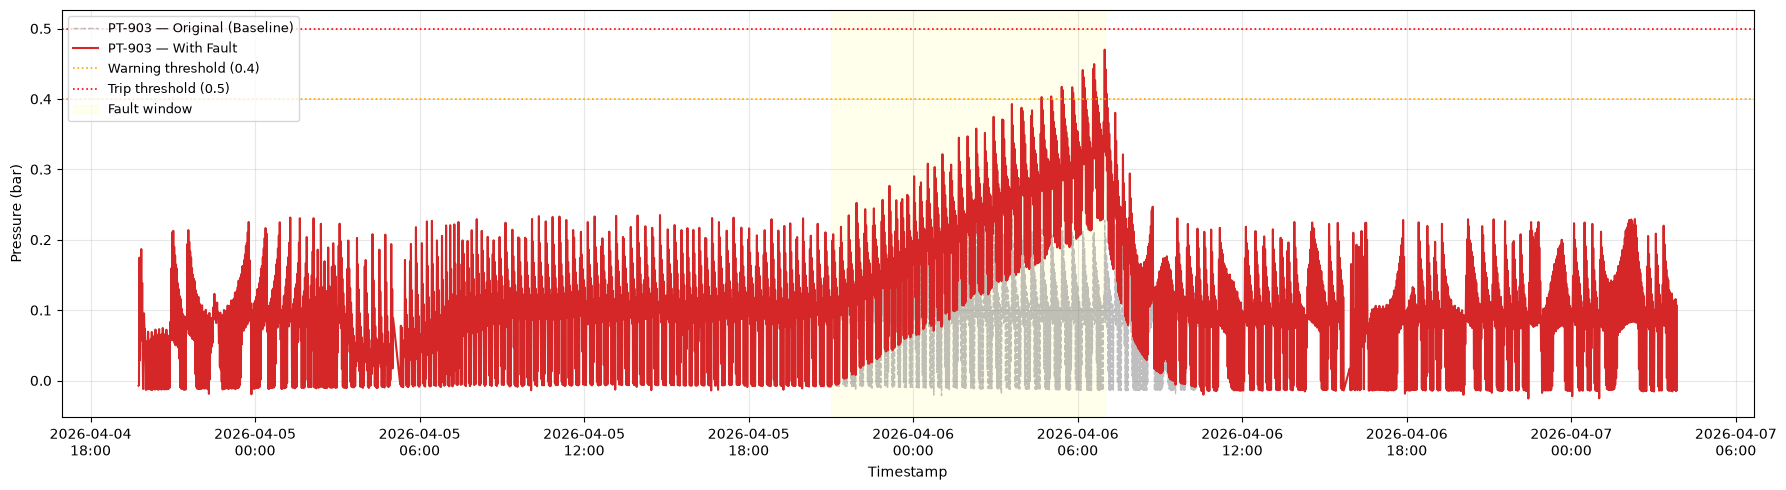
\includegraphics[width=0.95\textwidth]{imgs/fault_f1_medium_s16.png}
    \caption{F1 (clogged exhaust filters), medium severity: PT-903 with and without the injected fault. 
    The fault lasts 10 hours, starting 45\% of the way through the session.}
    \label{fig:fault_f1}
\end{figure}

\begin{figure}[htbp]
    \centering
    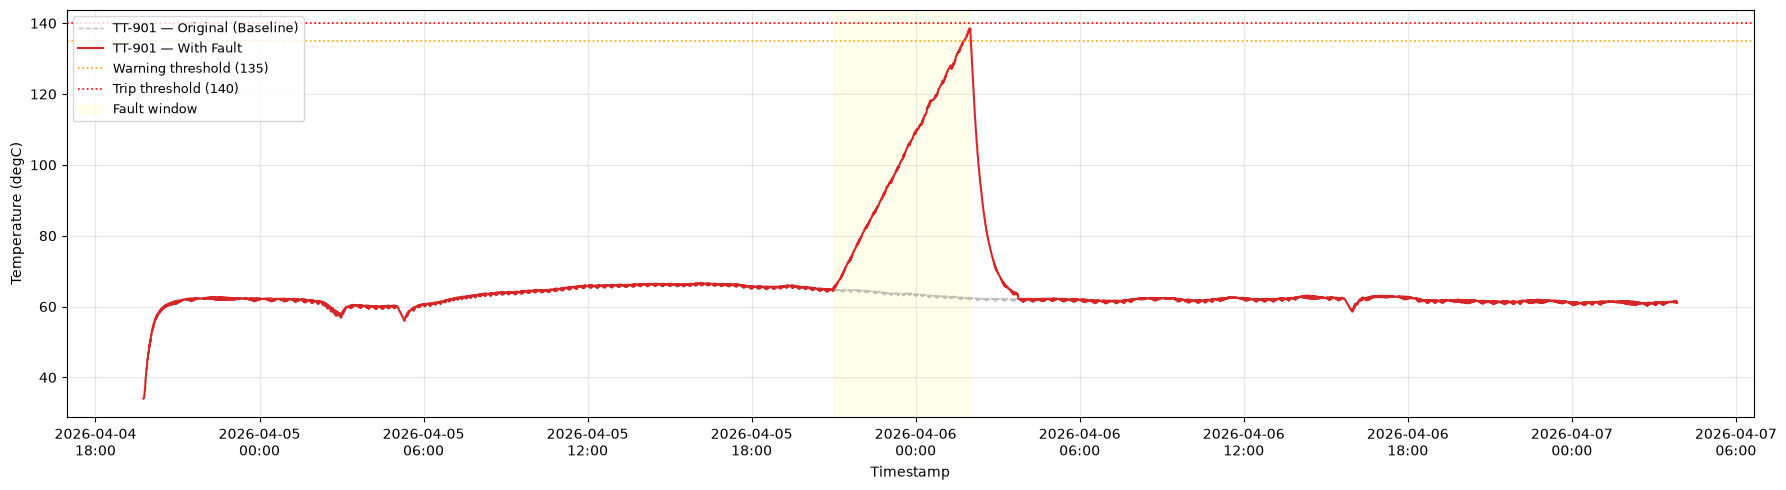
\includegraphics[width=0.95\textwidth]{imgs/fault_f2_medium_s16.png}
    \caption{F2 (insufficient cooling), medium severity: TT-901 with and without the injected fault. The 
    fault lasts 5 hours, starting 45\% of the way through the session.}
    \label{fig:fault_f2}
\end{figure}

\begin{figure}[htbp]
    \centering
    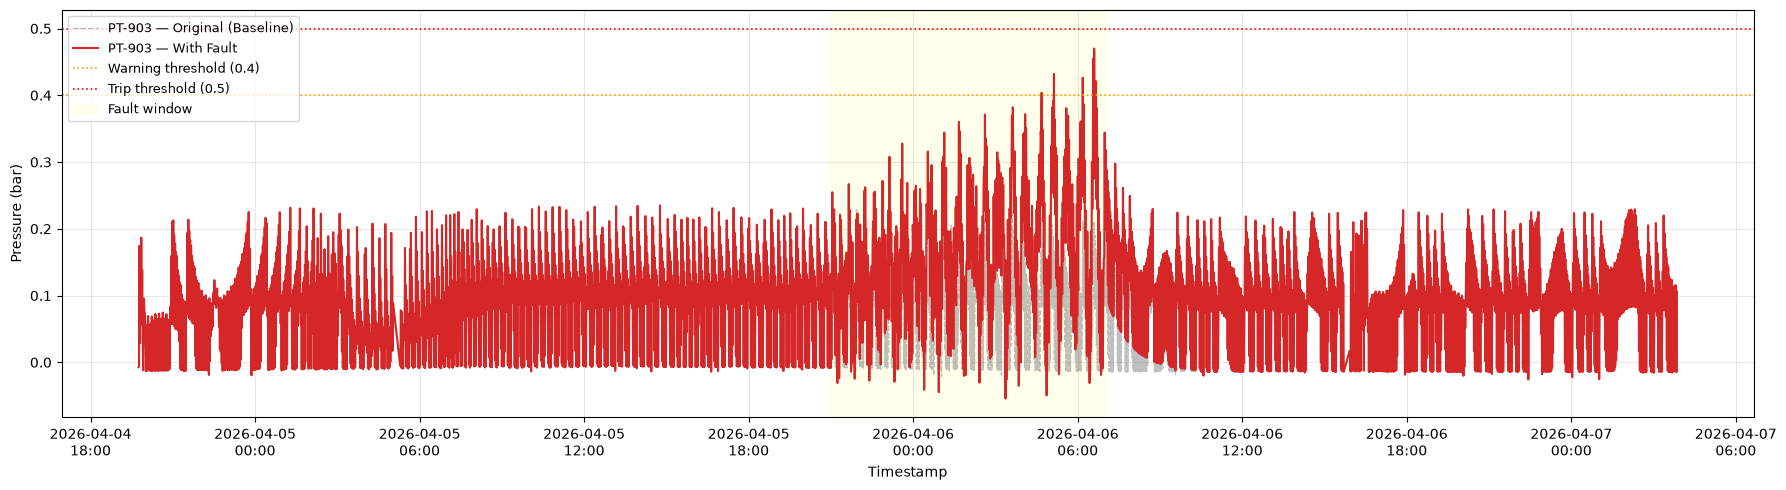
\includegraphics[width=0.95\textwidth]{imgs/fault_f3_medium_s16.png}
    \caption{F3 (float valve fault), medium severity: PT-903 with and without the injected fault, showing 
    the oscillatory pattern characteristic of this fault type. The fault lasts 10 hours, starting 45\% of 
    the way through the session.}
    \label{fig:fault_f3}
\end{figure}

\begin{figure}[htbp]
    \centering
    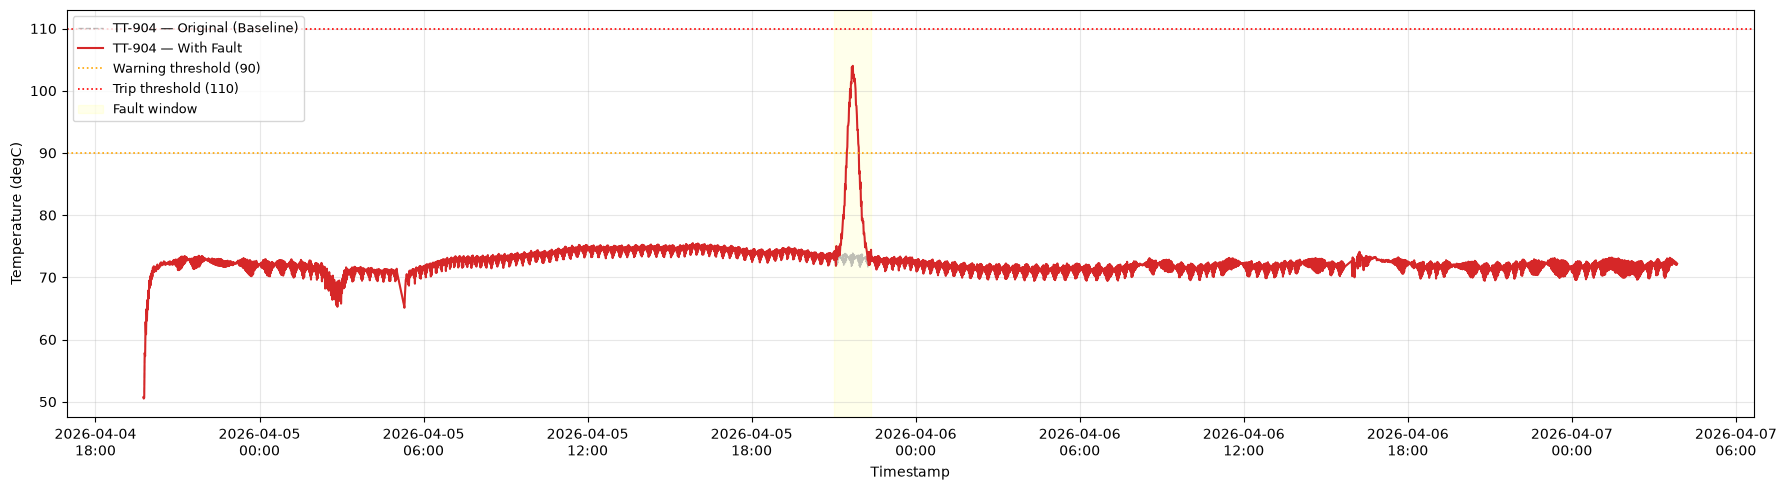
\includegraphics[width=0.95\textwidth]{imgs/fault_f4_medium_s16.png}
    \caption{F4 (defective bearing), medium severity: TT-904 with and without the injected fault, showing 
    the short, localized temperature spike characteristic of this fault type. The fault lasts about 1.4 
    hours, starting 45\% of the way through the session.}
    \label{fig:fault_f4}
\end{figure}

\subsection{Combined Fault Scenarios} \label{sec:fault_combined}

In addition to the four single fault scenarios, two combined fault scenarios were defined, each injecting 
two faults at the same time. These combinations test two different situations. Combo A combines F1 
(severe) and F3 (small), both affecting the same main sensor, PT-903, testing whether the models can still 
tell apart two fault mechanisms acting on a single signal at once. Combo B combines F2 (medium) and F4 
(severe), affecting two different but strongly correlated sensors, TT-901 and TT-904, testing whether the 
models can correctly attribute abnormal behaviour observed across multiple related sensors to two 
distinct faults occurring together.

The two combinations also differ in how their fault windows relate to each other in time. In Combo A, the 
F1 and F3 windows only partially overlap: F1 begins first and is still active when F3 starts, with the two 
overlapping for a limited period before F1 ends. In Combo B, the F4 window is fully contained within the 
longer F2 window, so F4 always occurs while F2 is already active. The resulting labelling scheme for both 
combined and false positive scenarios is described in Section~\ref{sec:fault_labeling}.

Figure~\ref{fig:fault_combo_a} illustrates Combo A, showing the partial overlap between the F1 and F3 
windows on the same sensor.

\begin{figure}[htbp]
    \centering
    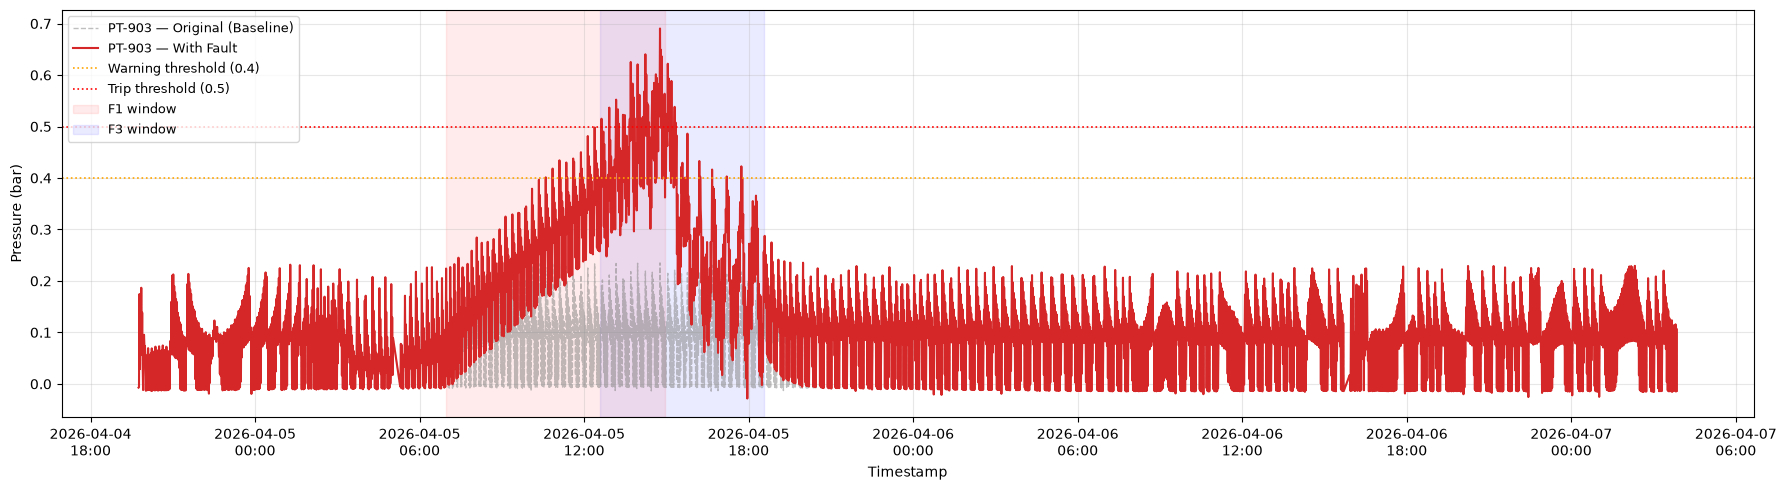
\includegraphics[width=0.95\textwidth]{imgs/fault_combo_a_s16.png}
    \caption{Combo A (F1 severe + F3 small): PT-903 with and without the injected faults, with the F1 and 
    F3 windows highlighted, showing their partial overlap in time.}
    \label{fig:fault_combo_a}
\end{figure}

\subsection{False Positive Scenarios} \label{sec:fault_fp}

To check whether the models can correctly avoid raising false alarms, a false positive scenario was also 
injected into each session: a brief, isolated Gaussian spike (10 to 12 minutes) in a single sensor during 
an otherwise normal period, kept below the sensor's trip threshold and, unlike the fault scenarios 
described above, not propagated to any correlated sensors. This represents a brief, physically implausible 
sensor deviation that does not correspond to any real equipment fault, and all such observations are 
labelled \texttt{false\_positive} rather than \texttt{normal}.

This scenario complements the frozen PT-903 sensor episode identified during exploratory data analysis, 
which was deliberately kept in the dataset as a naturally occurring, real world instance of the same 
concern.

\subsection{Anomaly Labeling Scheme} \label{sec:fault_labeling}

Every observation in the fault injected sessions carries four labels. A binary flag,
\texttt{is\_injected\_anomaly}, marks whether the observation falls inside any injected fault window. A
categorical \texttt{anomaly\_level} takes the value 0 for normal, 1 for incipient, or 2 for critical, based
on how the affected sensor's value compares to the manufacturer's warning and trip thresholds. For
small-severity faults this comparison is bypassed and the level is fixed at 1 for the whole fault window,
since by construction a small fault crosses the warning threshold but never reaches the trip threshold, 
applying the comparison observation by observation would otherwise
let normal fluctuation around the target push individual observations back below the warning threshold,
producing a label that alternates between 0 and 1 within a single continuous fault. A descriptive
\texttt{anomaly\_type} identifies which specific fault, or combination of faults, is responsible for the
observation. A continuous \texttt{severity\_score} additionally expresses the same severity levels
previously defined as a numeric value, to support the regression based formulation of the predictive
maintenance task: 0.33 for small faults, 0.67 for medium, and 1.0 for severe. Combined faults take the
maximum severity of their two constituent faults, and false positives are assigned 0.0, since they do not
represent genuine degradation.

For single fault scenarios, \texttt{anomaly\_type} simply takes the name of the fault 
(\texttt{clogged\_filters} for F1, \texttt{cooling\_fault} for F2, and so on). For combined fault 
scenarios, the label reflects how the two windows overlap in time. Outside any fault window, observations 
are labelled \texttt{normal}. Where only one fault is active, observations keep that fault's own label. 
Where both faults overlap, observations get a combined label naming both faults together (e.g. 
\texttt{clogged\_filters+valve\_fault}).

The false positive scenario is labelled on its own: affected observations get \texttt{anomaly\_type} equal 
to \texttt{false\_positive}, kept separate from both real faults and normal operation. Regardless of how 
close the injected spike gets to the trip threshold, \texttt{anomaly\_level} for these observations is 
always kept at 0, since they do not correspond to a real degradation of the equipment.

Table~\ref{tab:fault_data_totals} summarizes the total number of observations by \texttt{anomaly\_type} 
across the complete set of data used in this dissertation, that is, the sessions with no injected faults 
together with every fault scenario generated from the two fault injected sessions. The counts correspond 
to the compiled training and test datasets described in Section~\ref{sec:training_compilation}, and 
therefore already exclude the 498 observations of the frozen PT-903 episode that are removed from the 
training portion.

\begin{table}[htbp]
\centering
\caption{Total observations by anomaly type across the compiled training and test datasets.}
\label{tab:fault_data_totals}
\small
\begin{tabular}{lr}
\hline
\textbf{Anomaly type} & \textbf{Observations} \\
\hline
normal (no fault injected)                              & 29{,}594  \\
normal (fault injected sessions, outside fault windows) & 104{,}706 \\
clogged\_filters                                        & 4{,}138   \\
valve\_fault                                             & 3{,}898   \\
cooling\_fault                                           & 2{,}520   \\
bearing\_fault                                           & 404     \\
cooling\_fault+bearing\_fault                            & 360     \\
clogged\_filters+valve\_fault                            & 182     \\
false\_positive                                          & 24      \\
\hline
\textbf{Total} & \textbf{145{,}826} \\
\hline
\end{tabular}
\end{table}


\section{Train and Test Set Compilation} \label{sec:training_compilation}

Once the fault injection scenarios were generated, the final training and test datasets were assembled by 
combining the sessions with no injected faults with a selected subset of the fault injected files.

The nine sessions not used for fault injection contribute their entire length as normal data, 29{,}594 
observations in total, labelled \texttt{is\_injected\_anomaly=0}, \texttt{anomaly\_level=0}, and 
\texttt{anomaly\_type='normal'}.

For each of the fifteen fault scenarios (twelve single faults, two combined faults, and one false positive 
scenario), two versions exist, one generated from each of the two sessions used for fault injection. One 
version is assigned to the training set and the other to the test set, with the constraint that both 
versions of the same fault scenario can never end up on the same side of the split. This guarantees that 
every fault scenario the models are evaluated on in testing comes from data they were never exposed to 
during training for that specific fault, providing a stronger test of generalization than a split 
performed at the level of individual rows.

The assignment was performed randomly (seed 42), subject only to the constraint described above. 
Table~\ref{tab:fault_split} lists the resulting assignment for every fault scenario.

\begin{table}[htbp]
\centering
\caption{Random assignment of each fault scenario to the training and test sets (seed 42).}
\label{tab:fault_split}
\small
\begin{tabular}{lll}
\hline
\textbf{Fault scenario} & \textbf{Train} & \textbf{Test} \\
\hline
F1\_small   & Session 17 & Session 16 \\
F1\_medium  & Session 16 & Session 17 \\
F1\_severe  & Session 16 & Session 17 \\
F2\_small   & Session 16 & Session 17 \\
F2\_medium  & Session 17 & Session 16 \\
F2\_severe  & Session 17 & Session 16 \\
F3\_small   & Session 17 & Session 16 \\
F3\_medium  & Session 16 & Session 17 \\
F3\_severe  & Session 16 & Session 17 \\
F4\_small   & Session 16 & Session 17 \\
F4\_medium  & Session 16 & Session 17 \\
F4\_severe  & Session 17 & Session 16 \\
Combo A     & Session 16 & Session 17 \\
Combo B     & Session 16 & Session 17 \\
False positive & Session 17 & Session 16 \\
\hline
\end{tabular}
\end{table}

Before the training set is assembled, the observations belonging to the frozen PT-903 episode are removed 
from the fault files assigned to training. That episode occurs within Session 17, so it is inherited by 
every fault file generated from that session, amounting to 498 observations across the 6 such files that 
the split assigned to training. Removing them keeps the episode out of the training data entirely, which 
is what makes it usable as a genuinely unseen instrumentation fault when evaluating whether the anomaly 
detection models can be misled into raising a false positive, as intended in Section~\ref{sec:cleaning}. 
The episode is left untouched in the fault files assigned to the test set.

Combining the normal sessions with the fault files selected for training then yields a total of 85{,}889 
observations, of which 80{,}190 are labelled as negative (\texttt{is\_injected\_anomaly=0}) and 5{,}699 as 
positive, a pronounced class imbalance (roughly 93\% negative, 7\% positive) that is taken into account 
when selecting evaluation metrics in Section~\ref{sec:evaluation_metrics}. The corresponding test set is 
made up exclusively of the fifteen fault files assigned to testing and comprises 59{,}937 observations, of 
which 5{,}803 are positive. Note that, unlike the training set, the test set contains no data from the 
fault-free sessions: every observation in it comes from a session into which a fault was injected, with 
the negative examples corresponding to the periods lying outside the injected fault windows. This keeps 
the fault-free sessions available in full as training data, at the cost of the test set carrying a 
slightly higher proportion of positive examples than the training set.

Figure~\ref{fig:training_set_full} presents the resulting training set in full, grouped by sensor type, 
with the injected anomaly regions highlighted. The dashed vertical line marks the boundary between the 
normal sessions and the fault files appended afterwards.

\begin{figure}[htbp]
    \centering
    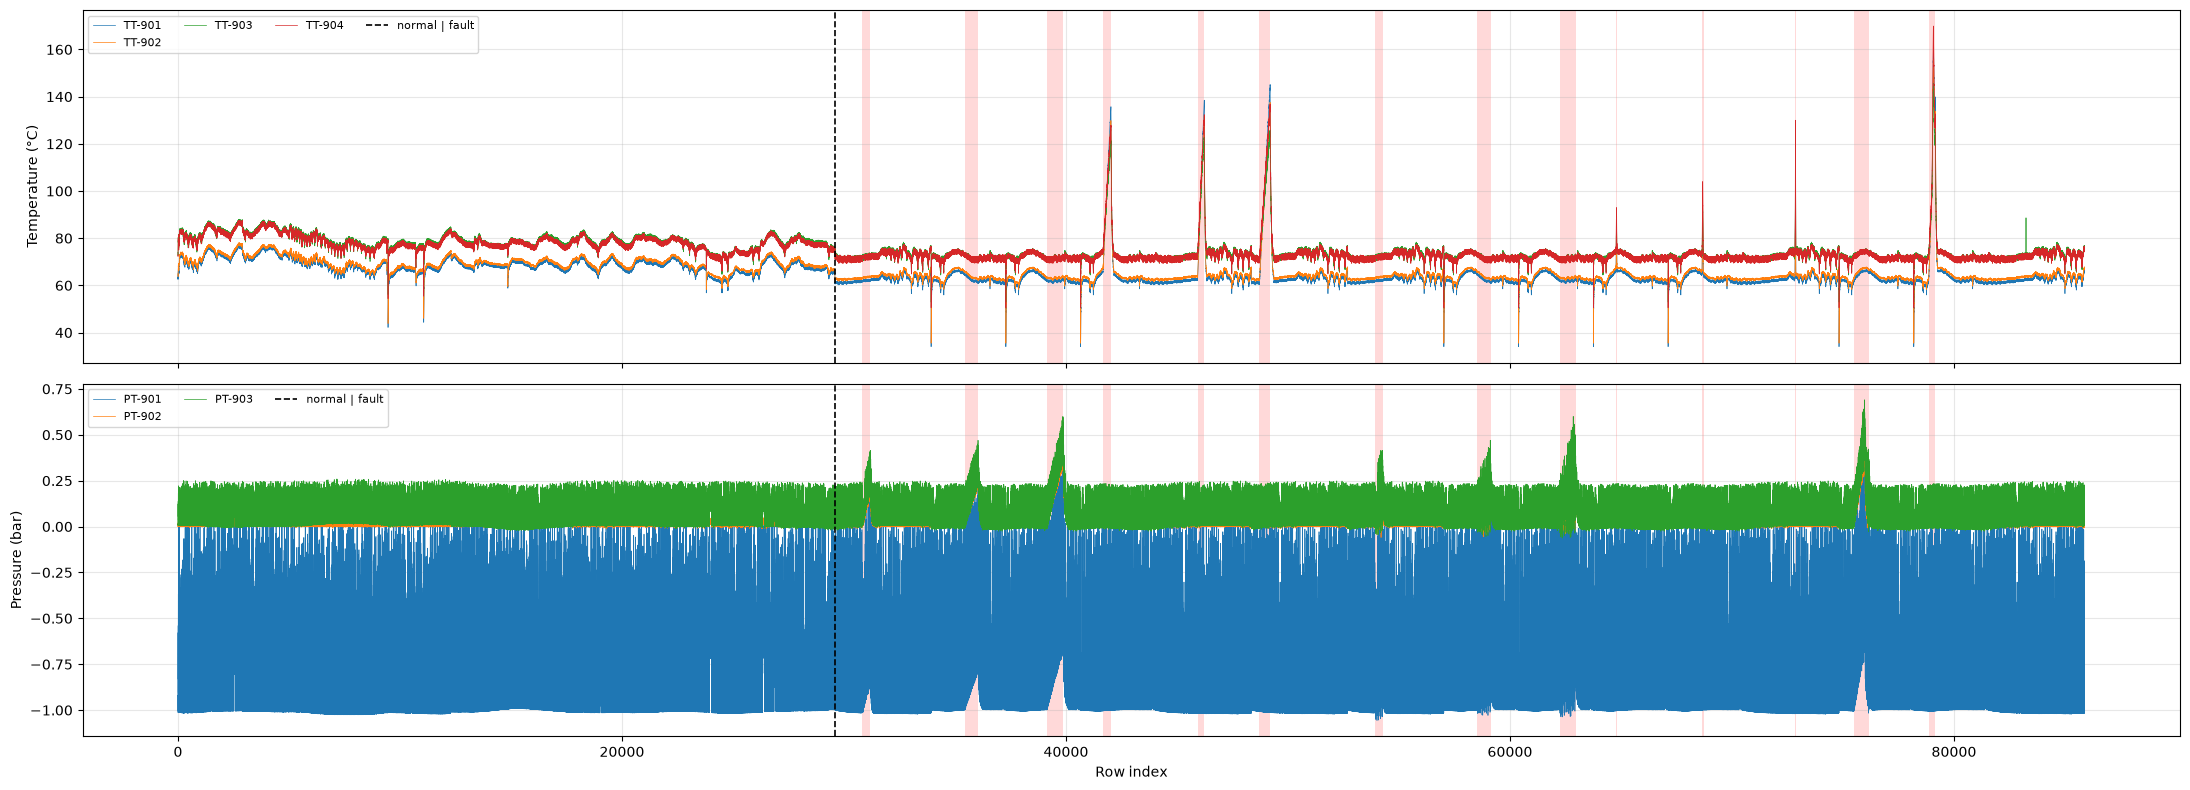
\includegraphics[width=0.95\textwidth]{imgs/training_set_full.png}
    \caption{Full compiled training set, grouped by sensor type, with injected anomaly regions shaded and 
    the boundary between normal sessions and fault files marked.}
    \label{fig:training_set_full}
\end{figure}

\section{Windowing} \label{sec:windowing}

To train and evaluate the models developed in this dissertation, the compiled dataset was 
segmented into fixed-length sliding windows. Each window consists of a fixed number of consecutive 
observations, and is labelled according to the state of its final (most recent) observation, so that a 
prediction always reflects the most up-to-date point in time given the preceding context.

Windows are constructed independently within each \texttt{source} (a single session, or a 
single fault-injected file), never spanning across the boundary between two sources. This mirrors the 
same principle already applied during data cleaning, where session boundaries 
prevent the fabrication of continuity across gaps or across genuinely distinct stretches of data: since 
different sources can correspond to different sessions, different fault scenarios, or different points in 
time altogether, a window spanning two of them would mix unrelated information as if it reflected a single 
continuous evolution of the process. Within each source, windows are extracted with a stride of one 
observation, so that consecutive windows overlap by all but one time step.

A wide range of window sizes was tested systematically, from 1 to 1{,}024 observations 
(1, 2, 4, 8, 16, 32, 64, 128, 256, 512, and 1{,}024 minutes), to characterize how the amount of temporal 
context available to each model affects its performance across the three tasks addressed in this 
dissertation. A window size of 1 corresponds to a model making a decision based solely on the current 
observation, with no temporal context at all, and serves as a baseline for measuring how much a longer context actually helps. 
A window size of 2{,}048 was initially considered but excluded from the 
final experiments, since only a small number of sources are long enough to yield a meaningful number of 
windows at that length, sharply reducing the amount of usable training and test data.

Sessions shorter than 1{,}000 observations were discarded during data cleaning, 
since they would not even fit a single window at the largest window size tested here, 1{,}024.

\section{Train/Validation Split and Normalization} \label{sec:data_split}

The assignment of entire sessions and fault scenarios to training and test data was already described: 
each of the fifteen fault scenarios has two versions, generated 
from two different sessions, with one version assigned to training and the other to testing, so that the 
models are always evaluated on a fault occurrence they were never exposed to during training. This 
section describes how a validation set is further carved out of the training data, used for model 
selection rather than for the final reported results, and how the data is normalized consistently with 
this split.

Since consecutive windows overlap by all but one time step, a validation 
split performed at the level of individual windows would place near-duplicate windows on both sides of 
the split, since two overlapping windows from the same source share almost all of their observations. 
This would let a model see, during validation, a window that is nearly identical to one already seen 
during training, producing an overly optimistic and misleading measure of generalization. To avoid this, 
every train/validation split in this dissertation is performed at the level of \texttt{source} rather than 
at the level of individual windows: all windows belonging to the same source are kept together on the same 
side of the split.

For the traditional machine learning baselines, model selection during 
hyperparameter search is performed using grouped cross-validation, with the training sources split into 
three folds. For the deep learning models, a 
single validation split is used instead, holding out 15\% of the training sources for validation. This 
validation set is used both to select the best hyperparameter configuration among those tested and to 
determine when to stop training.

All continuous process variables are standardized (zero mean, unit variance) before windowing. The 
mean and standard deviation used for this are computed only from the training data, and then applied 
to both the training and test data, so the test set is not used to compute the scaling.

\section{Task Formulation} \label{sec:task_formulation}

Building on the conceptual definitions of AD, FD, and PdM introduced in Chapter~\ref{chap:sota}, 
this section states how each task is formulated as a learning 
problem in this dissertation, in terms of its input, output, and problem type.

All three tasks share the same input: a fixed-length window of the fourteen continuous process variables, normalized as 
previously described. The three tasks 
differ only in what they predict from that window, and in how the corresponding prediction is scored.

AD is formulated as a binary classification problem: given a window, the model predicts 
whether its final observation corresponds to an injected fault (\texttt{is\_injected\_anomaly}), 
regardless of which specific fault is responsible or how severe it is.

FD is formulated as a multi-label classification problem rather than a multiclass one: the 
model predicts four independent binary outputs, one per fault type (clogged filters, insufficient 
cooling, float valve fault, and defective bearing), rather than a single label chosen from a fixed set of 
mutually exclusive classes. This choice follows directly from the combined fault scenarios described in 
Section~\ref{sec:fault_combined}, where two faults can be active at the same time: a multi-label 
formulation allows the corresponding two outputs to be predicted as active simultaneously, whereas a 
multiclass formulation would require treating every such combination as an entirely separate class, 
unrelated to its two constituent faults.

PdM is formulated as a regression problem over the continuous \texttt{severity\_score} 
introduced in Section~\ref{sec:training_compilation}, rather than as a classification problem over the 
discrete severity levels (small, medium, severe) used to define the fault scenarios themselves. This 
allows the models to express degradation as a continuous quantity, rather than being restricted to the 
three discrete levels used during fault injection.

For all three tasks, the prediction associated with a given window is taken to describe the state of the 
process at that window's final (most recent) observation, consistent with the windowing procedure 
previously described.

\section{Model Development} \label{sec:model_development}

This section describes the models developed and compared in this dissertation for the three tasks 
defined: traditional machine learning baselines, single task DL models and multi task DL architectures. 
All three families are trained and evaluated 
on the same compiled dataset and the same window sizes.

\subsection{Traditional Machine Learning Baselines} \label{sec:ml_baselines}

Two traditional machine learning algorithms were used as baselines: Random Forest and XGBoost. Both are 
widely used in the predictive maintenance literature reviewed in Chapter~\ref{chap:sota}, and represent 
two different ensemble strategies, bagging and boosting, providing a broader point of comparison than a 
single algorithm would. A Support Vector Machine was also initially considered, but was dropped from the 
final experiments due to poor scaling with the number of training samples.

Since these models cannot consume a sequence of observations directly, each window is instead summarized 
into a fixed set of statistics per sensor before being passed to them: the mean, standard deviation, 
minimum, maximum, and most recent value within the window. An alternative would have been to simply 
flatten each window into a single vector of raw values, but this was not adopted, since the number of 
resulting features would then grow directly with the window size, making the larger window sizes 
considerably harder to train on given the size of the training set. Summarizing each window into a fixed 
set of statistics instead keeps the number of input features constant across all window sizes tested.

For each combination of window size and task, both algorithms are tuned using a grid search 
over a small set of hyperparameters, listed in Table~\ref{tab:ml_baseline_grid}, using grouped 
cross-validation with three folds as described in Section~\ref{sec:data_split}. The best performing 
configuration on the validation folds is then retrained on the full training data and evaluated on the 
held-out test set.

\begin{table}[htbp]
\centering
\caption{Hyperparameter grid used for the traditional machine learning baselines.}
\label{tab:ml_baseline_grid}
\small
\begin{tabular}{lll}
\hline
\textbf{Model} & \textbf{Hyperparameter} & \textbf{Values tested} \\
\hline
Random Forest & Number of trees      & 100, 300 \\
              & Maximum tree depth   & 10, unlimited \\
XGBoost       & Number of estimators & 100, 300 \\
              & Maximum tree depth   & 3, 6 \\
\hline
\end{tabular}
\end{table}

For FD, both algorithms are adapted to the multi label formulation previously described. Random Forest supports multiple output 
labels natively, learning one tree ensemble internally for each fault type. XGBoost does not support this directly, and is instead 
wrapped so that one independent XGBoost model is trained per fault type, following the same hyperparameter 
configuration.

\subsection{Single-Task Deep Learning Models} \label{sec:stl_models}

For each of the three tasks a dedicated Long Short-Term 
Memory (LSTM) network is trained independently, receiving the same windowed input as the traditional 
baselines, but consuming it as a sequence rather than as a set of summary statistics.

All three single-task models share the same underlying architecture: an LSTM backbone reads the window 
one time step at a time, keeping only its output at the final time step, the one the prediction is made 
for. This output then passes through a single linear 
layer, which is the only part that changes across tasks: one output unit for AD, four 
independent output units for FD, and one output unit for PdM.

The three tasks also differ in their loss function, matching the problem type established. AD and FD,
both binary in nature, use binary cross-entropy with logits, applied independently to each of the four
outputs in the case of FD. Given the class imbalance already discussed, and the additional imbalance
across individual fault types noted (defective bearing in particular has substantially fewer positive
examples than the other three), the loss for both tasks is weighted per output using the square root of
the ratio between negative and positive examples in the training data, so that the network is not
encouraged to simply predict the majority class. The square root attenuates the weights of the rarest
outputs: applied unattenuated, a fault type present in well under one per cent of the training
observations would receive a weight large enough to dominate training and destabilise it. PdM, being a
regression task, uses the Huber loss with $\delta = 0.1$ instead, for the reasons given in
Section~\ref{sec:mtl_models}.

A separate model is trained for every combination of task and window size, following the same hyperparameter 
search and early stopping procedure that will be described. Figure~\ref{fig:stl_models} illustrates the three models side by side.

\begin{figure}[htbp]
\centering
\begin{tikzpicture}[
    block/.style={draw, rounded corners, minimum width=3.5cm, minimum height=0.85cm,
                  align=center, font=\small},
    shared/.style={block, fill=black!6},
    head/.style={block, fill=blue!12, very thick},
    io/.style={block, draw=black!55, dashed, fill=white},
    arrow/.style={-{Latex[length=2mm]}, thick},
    title/.style={font=\small\bfseries}
]

% dashed enclosure and common blocks, identical for the three models
\foreach \i/\x/\name in {0/0/{Anomaly Detection},
                         1/5.4/{Fault Detection},
                         2/10.8/{Predictive Maintenance}} {
    \draw[black!35, dashed, rounded corners]
        (\x-2.05,1.65) rectangle (\x+2.05,-5.15);
    \node[title] at (\x,1.15) {\name};
    \node[io]     (in\i)   at (\x,0)    {Input window};
    \node[shared] (lstm\i) at (\x,-1.6) {LSTM backbone};
    \draw[arrow] (in\i) -- (lstm\i);
}

% task-specific output layer, the only part that differs
\node[head] (fc0) at (0,-3.2)    {1 output};
\node[head] (fc1) at (5.4,-3.2)  {4 outputs};
\node[head] (fc2) at (10.8,-3.2) {1 output};

\node[io] (out0) at (0,-4.65)    {\scriptsize Is there a fault?};
\node[io] (out1) at (5.4,-4.65)  {\scriptsize Which of the 4 faults?};
\node[io] (out2) at (10.8,-4.65) {\scriptsize How severe? $[0,1]$};

\foreach \i in {0,1,2} {
    \draw[arrow] (lstm\i) -- (fc\i);
    \draw[arrow] (fc\i)   -- (out\i);
}
\end{tikzpicture}

\caption[Single-task deep learning models]{The three single-task models. Each is trained independently on
its own task and shares no weights with the others.}
\label{fig:stl_models}
\end{figure}

\subsection{Multi-Task Deep Learning Models} \label{sec:mtl_models}

In contrast to the single task models described, the multi task models 
developed in this dissertation use a single LSTM backbone shared across all three tasks, with the goal of 
allowing the network to learn a representation useful for all tasks simultaneously, rather than learning three separate representations independently. 
Two different ways of organizing the three task-specific output heads around this shared backbone are 
compared: a joint architecture and a cascaded architecture.

In the joint architecture, the three heads, anomaly, fault, and severity branch directly off the same 
shared representation produced by the LSTM, with no direct connection between them: each head only sees 
the shared backbone output and produces its prediction independently of what the other two heads predict.

In the cascaded architecture, the three heads are instead chained, so that each one also receives the 
predictions of the heads before it, mirroring a diagnostic reasoning process of first asking whether 
something is wrong, then what it is, and only then how severe it is. The anomaly head receives only the 
shared representation, as in the joint architecture. The fault head, however, receives the shared 
representation together with the anomaly head's predicted probability, and the severity head receives the 
shared representation together with both the anomaly probability and the four fault probabilities. This 
means that, unlike the joint architecture, the fault and severity heads in the cascaded architecture are 
conditioned on the outputs of the earlier heads, rather than only on the shared backbone.

In both architectures, the three heads are trained simultaneously, using a single combined loss that sums
the three task losses, each weighted by a fixed coefficient:

\begin{equation}
\mathcal{L} = w_{\text{anomaly}} \, \mathcal{L}_{\text{anomaly}} + w_{\text{fault}} \, \mathcal{L}_{\text{fault}} + w_{\text{severity}} \, \mathcal{L}_{\text{severity}}
\end{equation}

All three task losses are identical to those used by the corresponding single-task models: weighted
binary cross-entropy for anomaly and fault, and the Huber loss with $\delta = 0.1$ for severity. Keeping
them identical across the two families is deliberate, so that any difference observed between the
single-task and multi-task results can be attributed to the architecture rather than to the training
objective. The Huber loss is preferred over mean squared error for the severity head because the severity
score takes only four distinct values (0, 0.33, 0.67 and 1.0), so the residuals concentrate at a small
number of magnitudes. The Huber loss behaves quadratically for small residuals and linearly for large
ones, which prevents the observations whose severity is furthest from the prediction from dominating the
gradient. In the multi-task setting this matters more than in the single-task one, since an outsized
severity gradient would also pull the shared backbone away from the other two tasks.

The relative weights $w_{\text{anomaly}}$, $w_{\text{fault}}$, and $w_{\text{severity}}$ are kept fixed
rather than tuned as part of the hyperparameter search described, and are set separately for each
architecture: equal weighting for all three tasks in the cascaded architecture, and a weight of 1.30 on
the fault detection loss in the joint architecture, reflecting that task's comparatively slower
convergence when the three heads do not share any information between them. Figure~\ref{fig:mtl_models} compares the two architectures side by side.

\begin{figure}[htbp]
\centering
\resizebox{\textwidth}{!}{%
\begin{tikzpicture}[
    block/.style={draw, rounded corners, minimum width=1.9cm, minimum height=0.8cm,
                  align=center, font=\small},
    shared/.style={block, fill=black!6, minimum width=5.6cm},
    headb/.style={block, fill=blue!12, very thick},
    io/.style={block, draw=black!55, dashed, fill=white},
    arrow/.style={-{Latex[length=2mm]}, thick},
    chain/.style={-{Latex[length=2mm]}, thick, black!70},
    title/.style={font=\small\bfseries}
]

% both architectures share the same backbone and the same three heads
\foreach \p/\X/\name in {J/0/{Joint architecture}, C/9.2/{Cascaded architecture}} {
    \draw[black!35, dashed, rounded corners] (\X-4.0,1.6) rectangle (\X+4.0,-5.25);
    \node[title] at (\X,1.15) {\name};
    \node[io]     (in\p)   at (\X,0)    {Input window};
    \node[shared] (lstm\p) at (\X,-1.55){Shared LSTM backbone};
    \draw[arrow] (in\p) -- (lstm\p);

    \node[headb] (a\p) at (\X-2.7,-3.15) {Anomaly};
    \node[headb] (f\p) at (\X,-3.15)     {Fault};
    \node[headb] (s\p) at (\X+2.7,-3.15) {Severity};

    \node[io] (oa\p) at (\X-2.7,-4.7) {\scriptsize Is there\\[-2pt]\scriptsize a fault?};
    \node[io] (of\p) at (\X,-4.7)     {\scriptsize Which\\[-2pt]\scriptsize fault?};
    \node[io] (os\p) at (\X+2.7,-4.7) {\scriptsize How\\[-2pt]\scriptsize severe?};

    \draw[arrow] (lstm\p.south) -- (a\p.north);
    \draw[arrow] (lstm\p.south) -- (f\p.north);
    \draw[arrow] (lstm\p.south) -- (s\p.north);
    \draw[arrow] (a\p) -- (oa\p);
    \draw[arrow] (f\p) -- (of\p);
    \draw[arrow] (s\p) -- (os\p);
}

% the conditioning between heads is what distinguishes the cascaded architecture
\draw[chain] (aC) -- node[below, font=\tiny, inner sep=1.5pt] {$p_{a}$} (fC);
\draw[chain] (fC) -- node[below, font=\tiny, inner sep=1.5pt] {$p_{a},\,p_{f}$} (sC);
\end{tikzpicture}%
}

\caption[Multi-task deep learning architectures]{The two multi-task architectures. Both use a single LSTM
backbone shared by the three tasks and are trained with one combined loss. They differ only in the two
horizontal arrows: in the joint architecture each head sees only the shared representation, whereas in the
cascaded architecture the fault head additionally receives the predicted anomaly probability $p_{a}$, and
the severity head receives both $p_{a}$ and the four fault probabilities $p_{f}$.}
\label{fig:mtl_models}
\end{figure}

\subsection{Hyperparameter Tuning} \label{sec:hyperparameters}

All deep learning models developed in this dissertation follow the same hyperparameter search and stopping procedure.

For every combination of model and window size, six hyperparameter configurations are tried, varying the 
hidden size and number of layers of the LSTM backbone, together with the dropout rate and learning rate 
used for that configuration, as summarized in Table~\ref{tab:hyperparameter_grid}. Smaller hidden sizes 
are only combined with a single layer, since a network with very limited capacity is not expected to 
benefit from additional depth.

\begin{table}[htbp]
\centering
\caption{Hyperparameter configurations tried for every deep learning model.}
\label{tab:hyperparameter_grid}
\small
\begin{tabular}{rrrr}
\hline
\textbf{Hidden size} & \textbf{Layers} & \textbf{Dropout} & \textbf{Learning rate} \\
\hline
8  & 1 & 0.2 & 0.001  \\
16 & 1 & 0.2 & 0.001  \\
32 & 1 & 0.2 & 0.001  \\
32 & 2 & 0.4 & 0.001  \\
64 & 1 & 0.2 & 0.0005 \\
64 & 2 & 0.4 & 0.0005 \\
\hline
\end{tabular}
\end{table}

Each configuration is trained using the validation split described, with the Adam optimizer and a batch
size of 128 observations, for a maximum of 200 epochs. Early stopping is applied based on the validation
loss: if the validation loss does not improve for 20 consecutive epochs, training stops and the model's
weights are reverted to those of the epoch with the lowest validation loss observed, rather than the last
epoch trained. This avoids continuing to train a model past the point where it stops generalizing better,
and avoids selecting an over trained model over a better performing earlier one. In practice the
early-stopping criterion is reached well before the 200-epoch ceiling for the large majority of
configurations, so the maximum acts as a safeguard rather than as the operative stopping rule.

Only the configuration with the lowest validation loss is kept. This is the one evaluated on the test set 
and reported as the result for that model and window size. The other configurations are discarded.

\section{Evaluation Metrics} \label{sec:evaluation_metrics}

This section describes the metrics used to evaluate all models developed in this dissertation. A distinct 
set of metrics is used for each of the three tasks, reflecting the problem type each one was formulated 
as in Section~\ref{sec:task_formulation}. The same metrics, computed in the same way and on the same 
held-out test set, are applied to the traditional ML baselines, the single-task models, and 
the multi-task architectures, so that the three families remain directly comparable.

For AD, formulated as a binary classification problem, 
accuracy, precision, recall, F1-score, and the area under the ROC curve are reported. Given the class 
imbalance already discussed, accuracy alone is not a reliable 
indicator of performance, since a model that always predicts the majority class would still achieve a 
high accuracy without correctly identifying any faults. Precision, recall, and F1-score are therefore 
given more weight when comparing models. A fixed decision threshold of 0.50 is applied to the model's 
predicted probability to obtain a binary prediction, uniformly across all model families.

For FD, formulated as a multi-label classification problem, precision, recall, and F1-score 
are computed independently for each of the four fault types, using the same 0.50 decision threshold 
applied to each output. Since not every fault type is necessarily present in a given portion of the test 
data, an overall F1-score is also reported as the mean of the per-label F1-scores, computed only over the 
fault types that have at least one positive example in the data being evaluated, following the labelling 
scheme described.

For PdM, formulated as a regression problem over the continuous severity score, 
mean absolute error (MAE), root mean squared error (RMSE), and the 
coefficient of determination ($R^2$) are reported. MAE and RMSE express the average prediction error in 
the same units as the severity score itself, while $R^2$ indicates how much of the variation in severity 
is explained by the model, relative to always predicting the mean severity observed in the training data.